\section{Unity}
Glavno sučelje Unity platforme se može vidjeti na slici \ref{fig:unitysucelje}. Raspored koji se može vidjeti je optimalniji za rad ukoliko programer ima samo jedan monitor. U slučaju da programer ima više monitora onda bi se mogao napraviti puno pregledniji raspored. 
\subsection{Korisničko sučelje}
\subsubsection{Inspektor}
Inspektor (\emph{eng.~Inspector}) je dio korisničkog sučelja koji se koristi za provjeravanje pojedinih opcija komponenta igrajućih objekata (\emph{eng.~GameObject}). Pomoću njega je moguće dodavati elemente i obavljati operacije nad njima, te vidjeti sve moguće stavke o objektu.

\begin{figure}[h]
	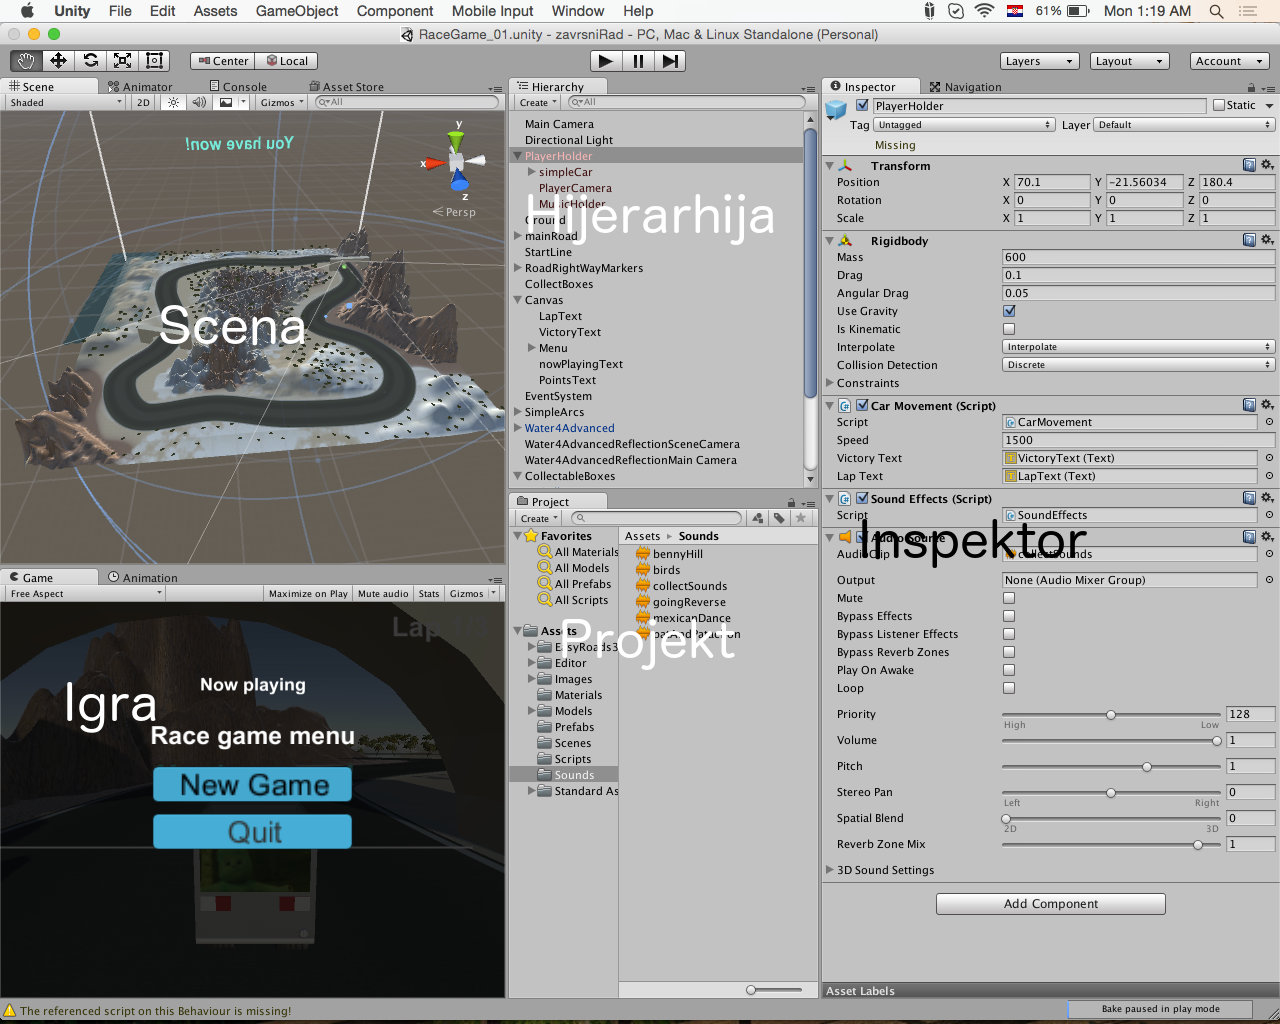
\includegraphics[width=12.5cm, height=10cm]{unitysucelje.png}
	\centering
	\caption{Unity sučelje}
	\label{fig:unitysucelje}
\end{figure}
\newpage

\subsubsection{Scena}
Scena (\emph{eng.~Scene}) se koristi prilikom izrade igre kako bi se moglo iz neutralne pozicije gledati cijeli svijet. Sve preinake koje se rade u svijetu kao što su dodavanje objekata, određivanje položaja, dimenzija se obavljaju unutar ovog dijela. Na slici \ref{fig:unitysucelje} u gornjem desnom kutu se može vidjeti maleni objekt koji je crvene, zelene i plave boje. On programeru govori trenutnu orijentaciju u svijetu. Zelena boja je y, crvena je x, a plava z koordinata.

\subsubsection{Hijerarhija}
Hijerarhija (\emph{eng.~Hierarchy}) je dio u kojem se nalaze svi igrajući objekti koji su napravljeni. Ovdje je moguće vidjeti odnos svih igrajućih objekata. Pod odnos se misli na odnos roditelj, dijete, gdje jedan igrajući objekt može biti dijete drugog. Na ovaj način je moguće iz roditelja pristupati djeci i njihovim komponentama. Iako Unity pruža mogućnost i obrnutog procesa, ovo ugnježđivanje omogućuje jednu odličnu funkcionalnost koja se koristi u igri. Ako je kamera dijete nekog objekta koji se pokreće sa nekom silom, tada kamera prati kretanje tog igrajućeg objekta i dobiva se iluzija kao u 3D igricama gdje se glavni junak gleda iz trećeg lica. 

\subsubsection{Projekt}
Projekt (\emph{eng.~Project}) segment omogućava programeru da vidi sve datoteke koje su uključene u igru i njihovu hijerarhiju. Zbog praktičnosti se naprave direktoriji za skripte, zvukove, modele i ostale objekte koji će se ponavljati kroz igru, kako bi se što lakše mogli pronaći prilikom rada. Postoji ugrađeni pretraživač za još jednostavnije pronalaženje željenih datoteka, kao i različiti filteri.

\subsubsection{Igra}
Ovaj dio je ono što igrač vidi kada pokrene igru, a omogućava programeru da što zornije postavi parametre kako bi igra izgledala kako je on zamislio. Moguće je postaviti da se prilikom pokretanja igre u Unity platforma poveća slika na maksimum (\emph{eng.~ maxmize on play}). Pokretanje igre je kao slušanje glazbe u bilo kojem alatu. Postoje igraj (\emph{eng.~play}), pauziraj i pomak po slici.

\subsubsection{Konzola}
Konzola (\emph{eng.~Console}) se koristi za provjeravanja k\^oda unutar igre. Moguće je ispisivati logove za provjeru pojedinih varijabli tokom igranja i provjeravanja okidača \emph{eng.~Trigger}  da li uistinu rade. Bilo koja greška koja nije uzrokovana tijekom rada će prvo biti prikazana u konzoli crvenom bojom sa oznakom linije i imenom skripte u kojoj se dogodila greška. Konzolu je moguće vidjeti na slici \ref{fig:konzolaStore}.

\subsubsection{Trgovina}
Trgovina (\emph{eng.~Asset Store}) se koristi za kupnju ili nabavljanje gotovih modela preko interneta, koje je netko drugi već napravio. U slučaju ove igre, cesta je preuzeta sa trgovine jer sama izrada ceste bi bio preduogtrajan proces. Trgovina ima svoje filtere za pojedine kategorije igara i tipova objekata koji su potrebni. Trgovina se može vidjeti na slici \ref{fig:konzolaStore}.

\begin{figure}[h]
	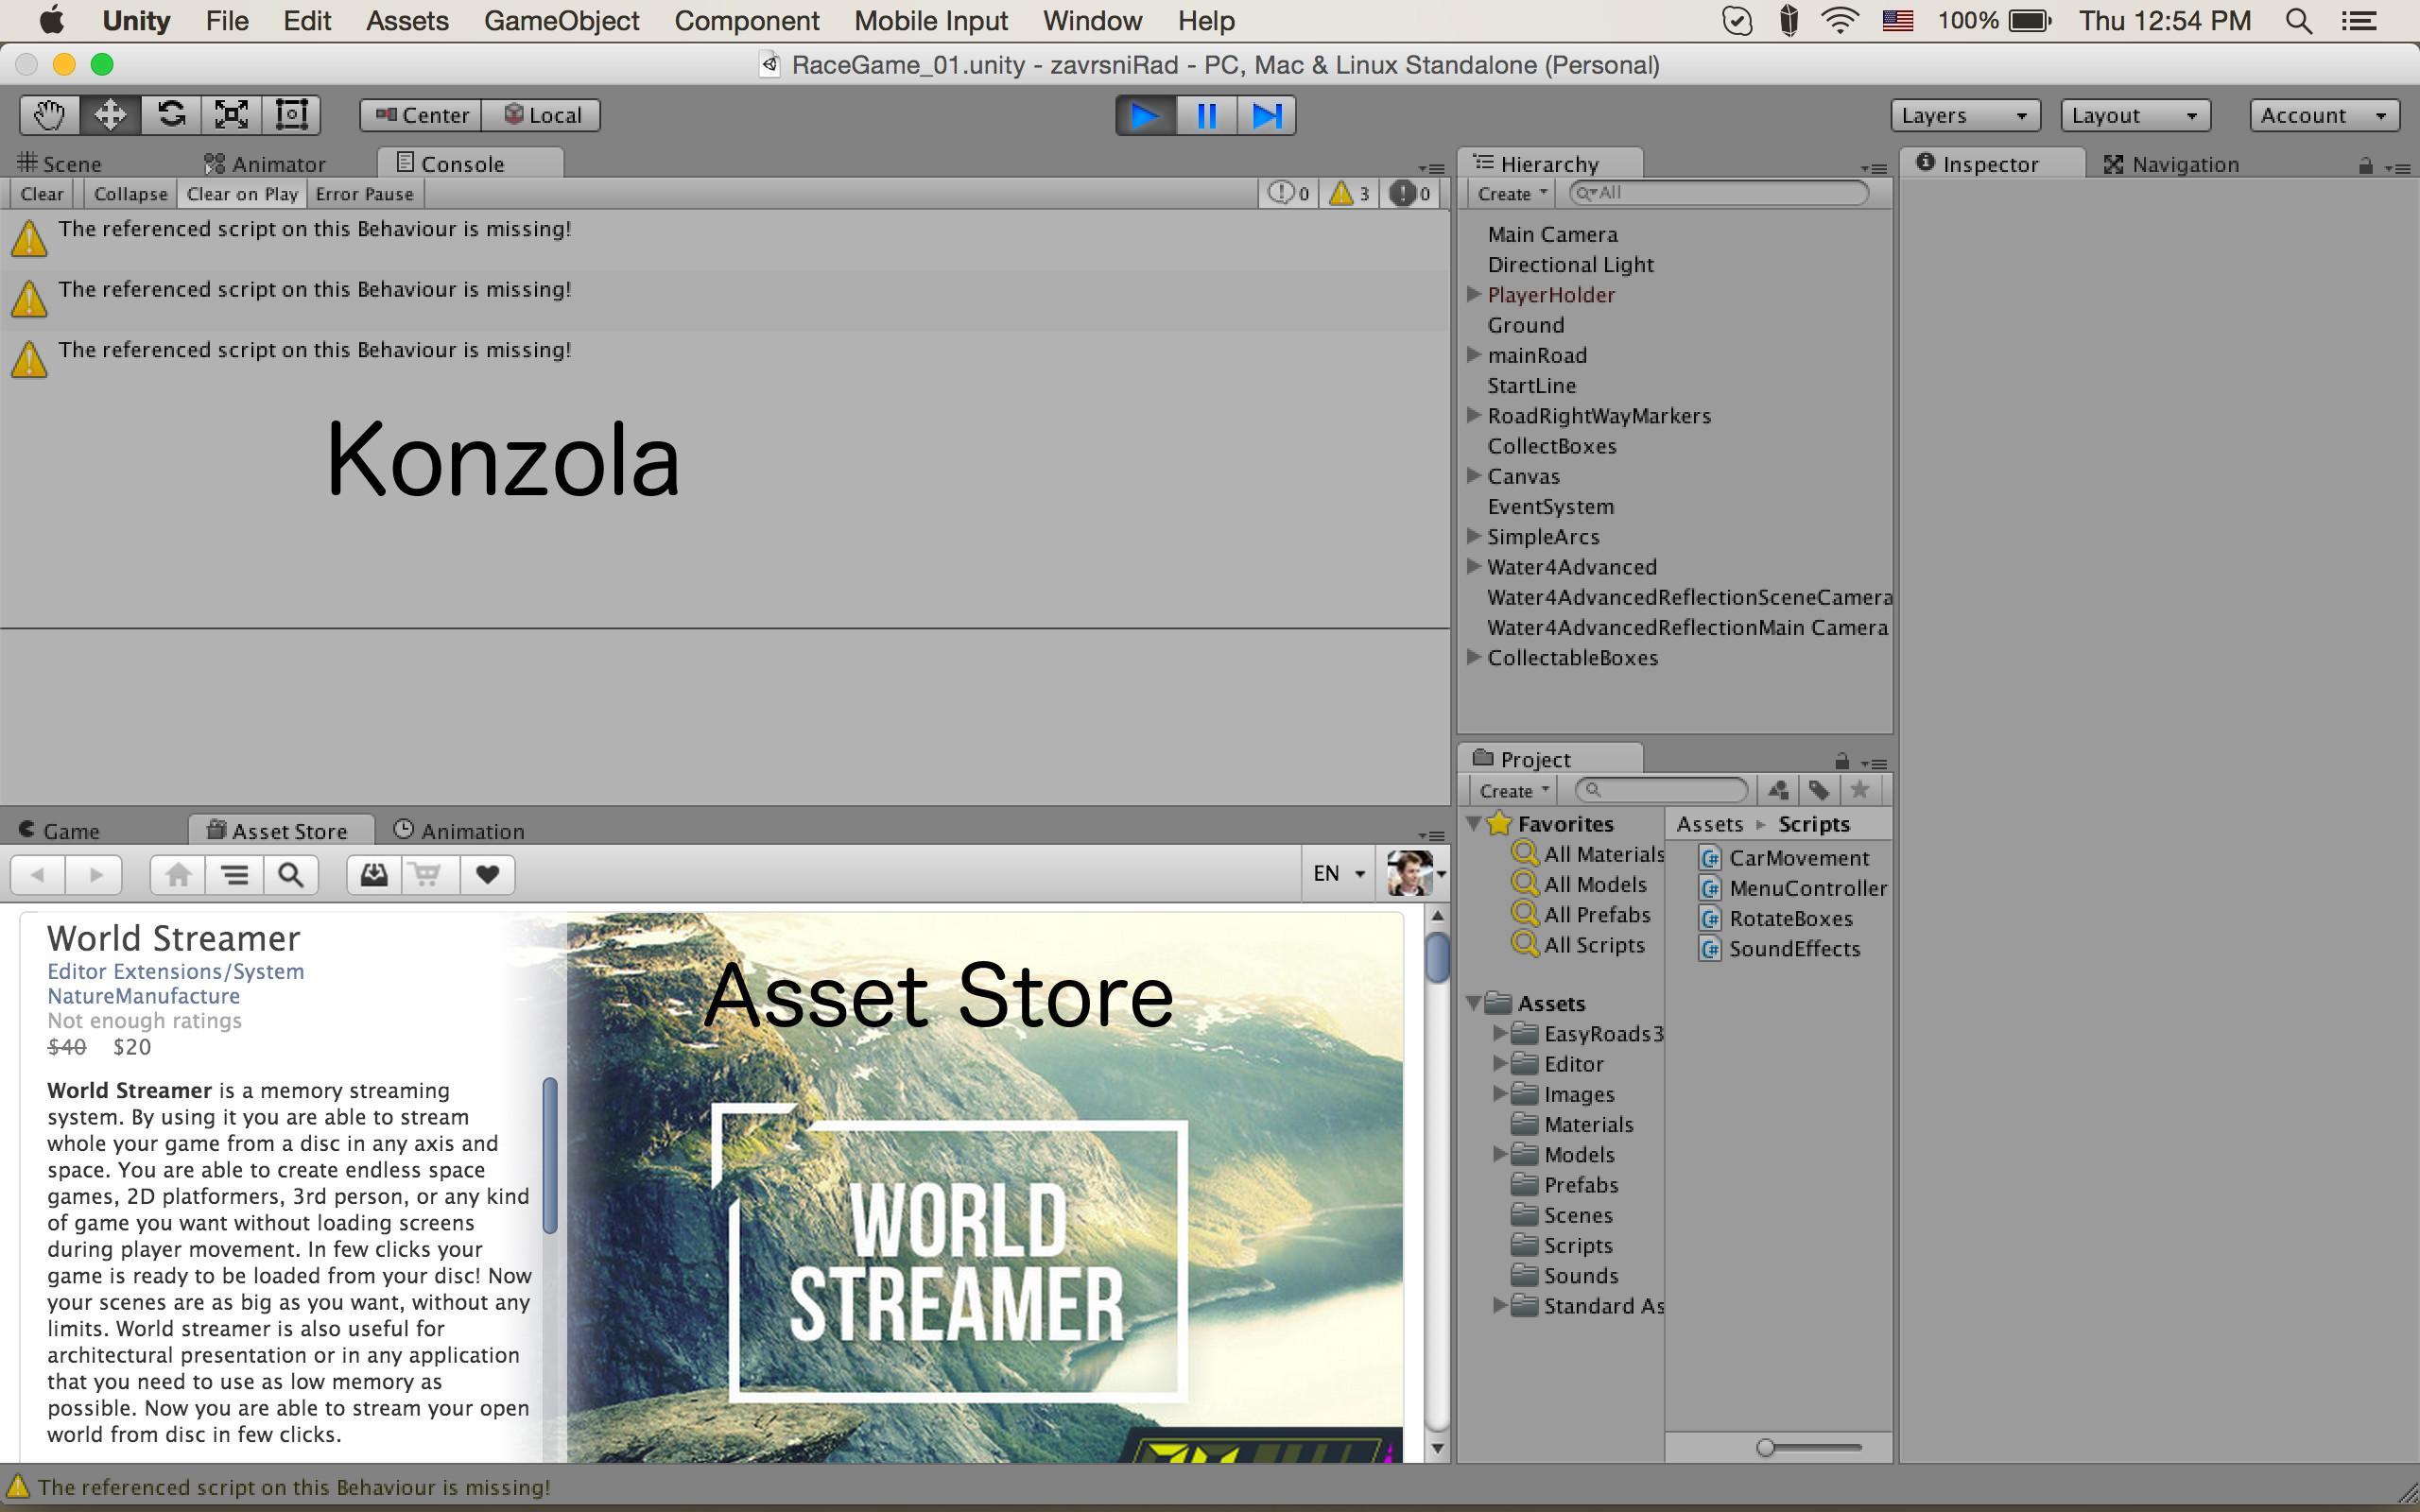
\includegraphics[width=12.5cm, height=10cm]{konzola_store.jpg}
	\centering
	\caption{Konzola i sučelje}
	\label{fig:konzolaStore}
\end{figure}

\subsection{Igrajući objekti}
Svaki objekt koji se može vidjeti u unity-u je \textbf{igrajući objekt}. Kada se napravi bilo koji objekt on treba imati svoju poziciju unutar svijeta. Kako bi se mogla znati njegova pozicija koristimo komponente. Svaki objekt mora imati svoju transformaciju (\emph{eng.~ Transform}). U suštini igrajući objekti su samo kontejneri koji sadrže komponente.

\subsection{Kamera}
Kamere se koriste za prikaz igre. Koristeći više kamera moguće je napraviti različite efekte i animacije za igrača, te stvoriti jedinstveno iskustvo tijekom igranja igre. Kamere imaju dvije moguće projekcije (ortografijsku i perspektivnu). Ortografijska se koristi za 2D igrice ili ako nije bitna dubina u igricama. Najčešće su to neke platformske igre, puzzle ili slično. Perspektivna se koristi ako želimo pokazati dubinu u igri. U ovoj igri se koristi perspektivna projekcija, te je postavljena kao dijete automobilskog igrajućeg objekta. Na ovaj način kamera slijedi automobil i dobiva se pravo iskustvo vožnje automobila.
\subsection{Svijetlo}
Svijetla se naravno koriste za osvijetljavanje svijeta, ali i za stvaranje ugođaja. Moguće je mijenjati boje svijetla, te tako stvarati prekrasne ambijente. Može se definirati spektar, doseg, boja, tip, intenzitet, intenzitet odbijanja, sjena i ostale naprednije funkcije. Zanimljivo je što se može definirati da svjetlo ne baca sjenu za igrajuće objekte.

Za bolju funkcionalnost se može preko padajućeg izbornika na svijetlu postaviti da je već ispečeno (\emph{eng.~Baked}). Ovo znači da će se sva svijetla prilikom pokretanja igre izračunati i postaviti za igrajuće objekte koji se ne kreću. Ovo je veoma praktično jer nema potrebe preračunavati za te objekte utjecaj sa svjetlom, već će se to obavljati ukoliko pokraj njega dođe ne-statičan objekt.
\newpage

\subsection{Montažni objekti}
Montažni objekt (\emph{eng.~Prefab}) je objekt koji je već napravljen, te se želi multiplicirati više puta. Ako se koristi više istih igrajućih objekata, kao na primjer više istih automobila koji dijele sve funkcionalnosti, tada nije praktično raditi promjene nad svakim automobilom zasebno, te se zato koriste montažni objekti. Kada se napravi novi igrajući objekt može se od njega napraviti montažni objekt preko izbornika \emph{Asset}, pa zatim \emph{Create Prefab}. Nakon što se napravi montažni objekt može se jednostavno povlačiti u svijet, te tako stvarati nove instance igrajućih objekata, koje dijele iste funkcionalnosti. Sada ako se nešto želi promijeniti, može se mijenjati bilo koji od objekata i Unity će pitati da li treba primjeniti ove promjene i na ostale instance ovog montažnog objekta.

\subsection{Komponente}
Komponente su dijelovi igrajućih objekata. One daju funkcionalnost objektima, te omogućavaju krajnjim korisnicima da razlikuju igrajuće objekte. Neke važnije komponente koje su korištene za izradu igrice su:

\begin{itemize} 
	\item Kruta tijela
	\item Sudarači
	\item Transformacija
	\item Kolni sudarači 
\end{itemize}

\subsubsection{Kruta tijela}
Kruta tijela (\emph{eng.~Rigid Body}) igrajućim objektima daju ponašanje kao u stvarnom svijetu. Objektima daju dodatne informacije kao što su na primjer masa, primjena sile za pomicanje objekata, hoće li vjetar utjecati na kretanje i tako dalje. Dodavajući kruta tijela može se definirati hoće li gravitacija utjecati na element. U igri je najvažnija informacija bila masa zbog bolje simulacija pravog automobila.
\subsubsection{Sudarači}
Sudarači (\emph{eng.~ Colliders}) su komponente koje omogućavaju igrajućim objektima fizičku koliziju. Oni se ne mogu vidjeti tokom igranja igre, a i nisu zbog toga napravljeni. Postoji više oblika sudarača (kvadar, sfera, kapsula, krug...) i svaki od njih se koristi za aproksimiranje mreže igrajućih objekata. Moguće je dodati sudarač tako da se savršeno slaže sa mrežom igrajućeg objekta, ali tada bi gubili na performansi. Način za bolju aproksimaciju je korištenje konveksnih (\emph{eng.~Convex}) sudarača.

Unity u svakom trenutku provjerava da li je sudarač imao koliziju sa nekim drugim igrajućim objektom koji isto ima svoj sudarač. Kada bi se oblik postavio da savršeno odgovara mreži igrajućeg objekta, tada bi trebalo obavljati previše računanja. U igri se sudarač u obliku kvadra za tijelo modela jer veoma dobro aproksimira automobil, a za kotače se koriste kolni sudarači.

Unity ima predefinirane elemente za simulaciju pravih kotača prizemljenih vozila koje zovemo \textbf{kolni sudarači} (\emph{eng.~Wheel Colliders}). Prema dokumentaciji Unity platforme ovi sudarači se ne dodaju kao komponente, već trebaju biti komponente zasebnih igrajućih objekata. Znači za svaki kotač treba napraviti novi igrajući objekt, koji se zove prazni igrajući objekt (\emph{eng.~Empty GameObject}), te se komponenta doda praznom objektu. Cijeli igrajući objekt se pomakne tako da je centriran sa kotačima.

Najvažnije metode za vožnju su moment motora (\emph{eng.~Motor Torque}), moment kočnice (\emph{eng.~Brake Torque}), te kut okretanja (\emph{eng.~Steer Angle}). Moment motora je sila koja djeluje na osovinu kotača izražena u Newton metrima. Predznak sile će odrediti smjer kretanja. Kut okretanja određuje za koliko će se okrenuti model prilikom skretanja, a moment kočnice određuje silu kočenja u Newton metrima. Primjer k\^oda za kretanje vozila se može vidjeti u ispisu \ref{kretanjeVozila}

\begin{lstlisting}[caption={Skripta za kretanje vozila}, label=kretanjeVozila]
for(int i = 0; i < 4; i++)
    this.wheelsColliders[i].motorTorque = thrustTorque;
\end{lstlisting}

Jedan propust postoji kod ovih sudarača. Naime, ukoliko se postave veće brzine kretanja model sam počinje skretati prema desno. Prema forumima Unity društva više je rješenja, iako nijedno od njih nije pomoglo u ovoj igri. Rješenje koje je primjenjeno u ovoj igri je optimizirana brzina.

\begin{figure}[h]
	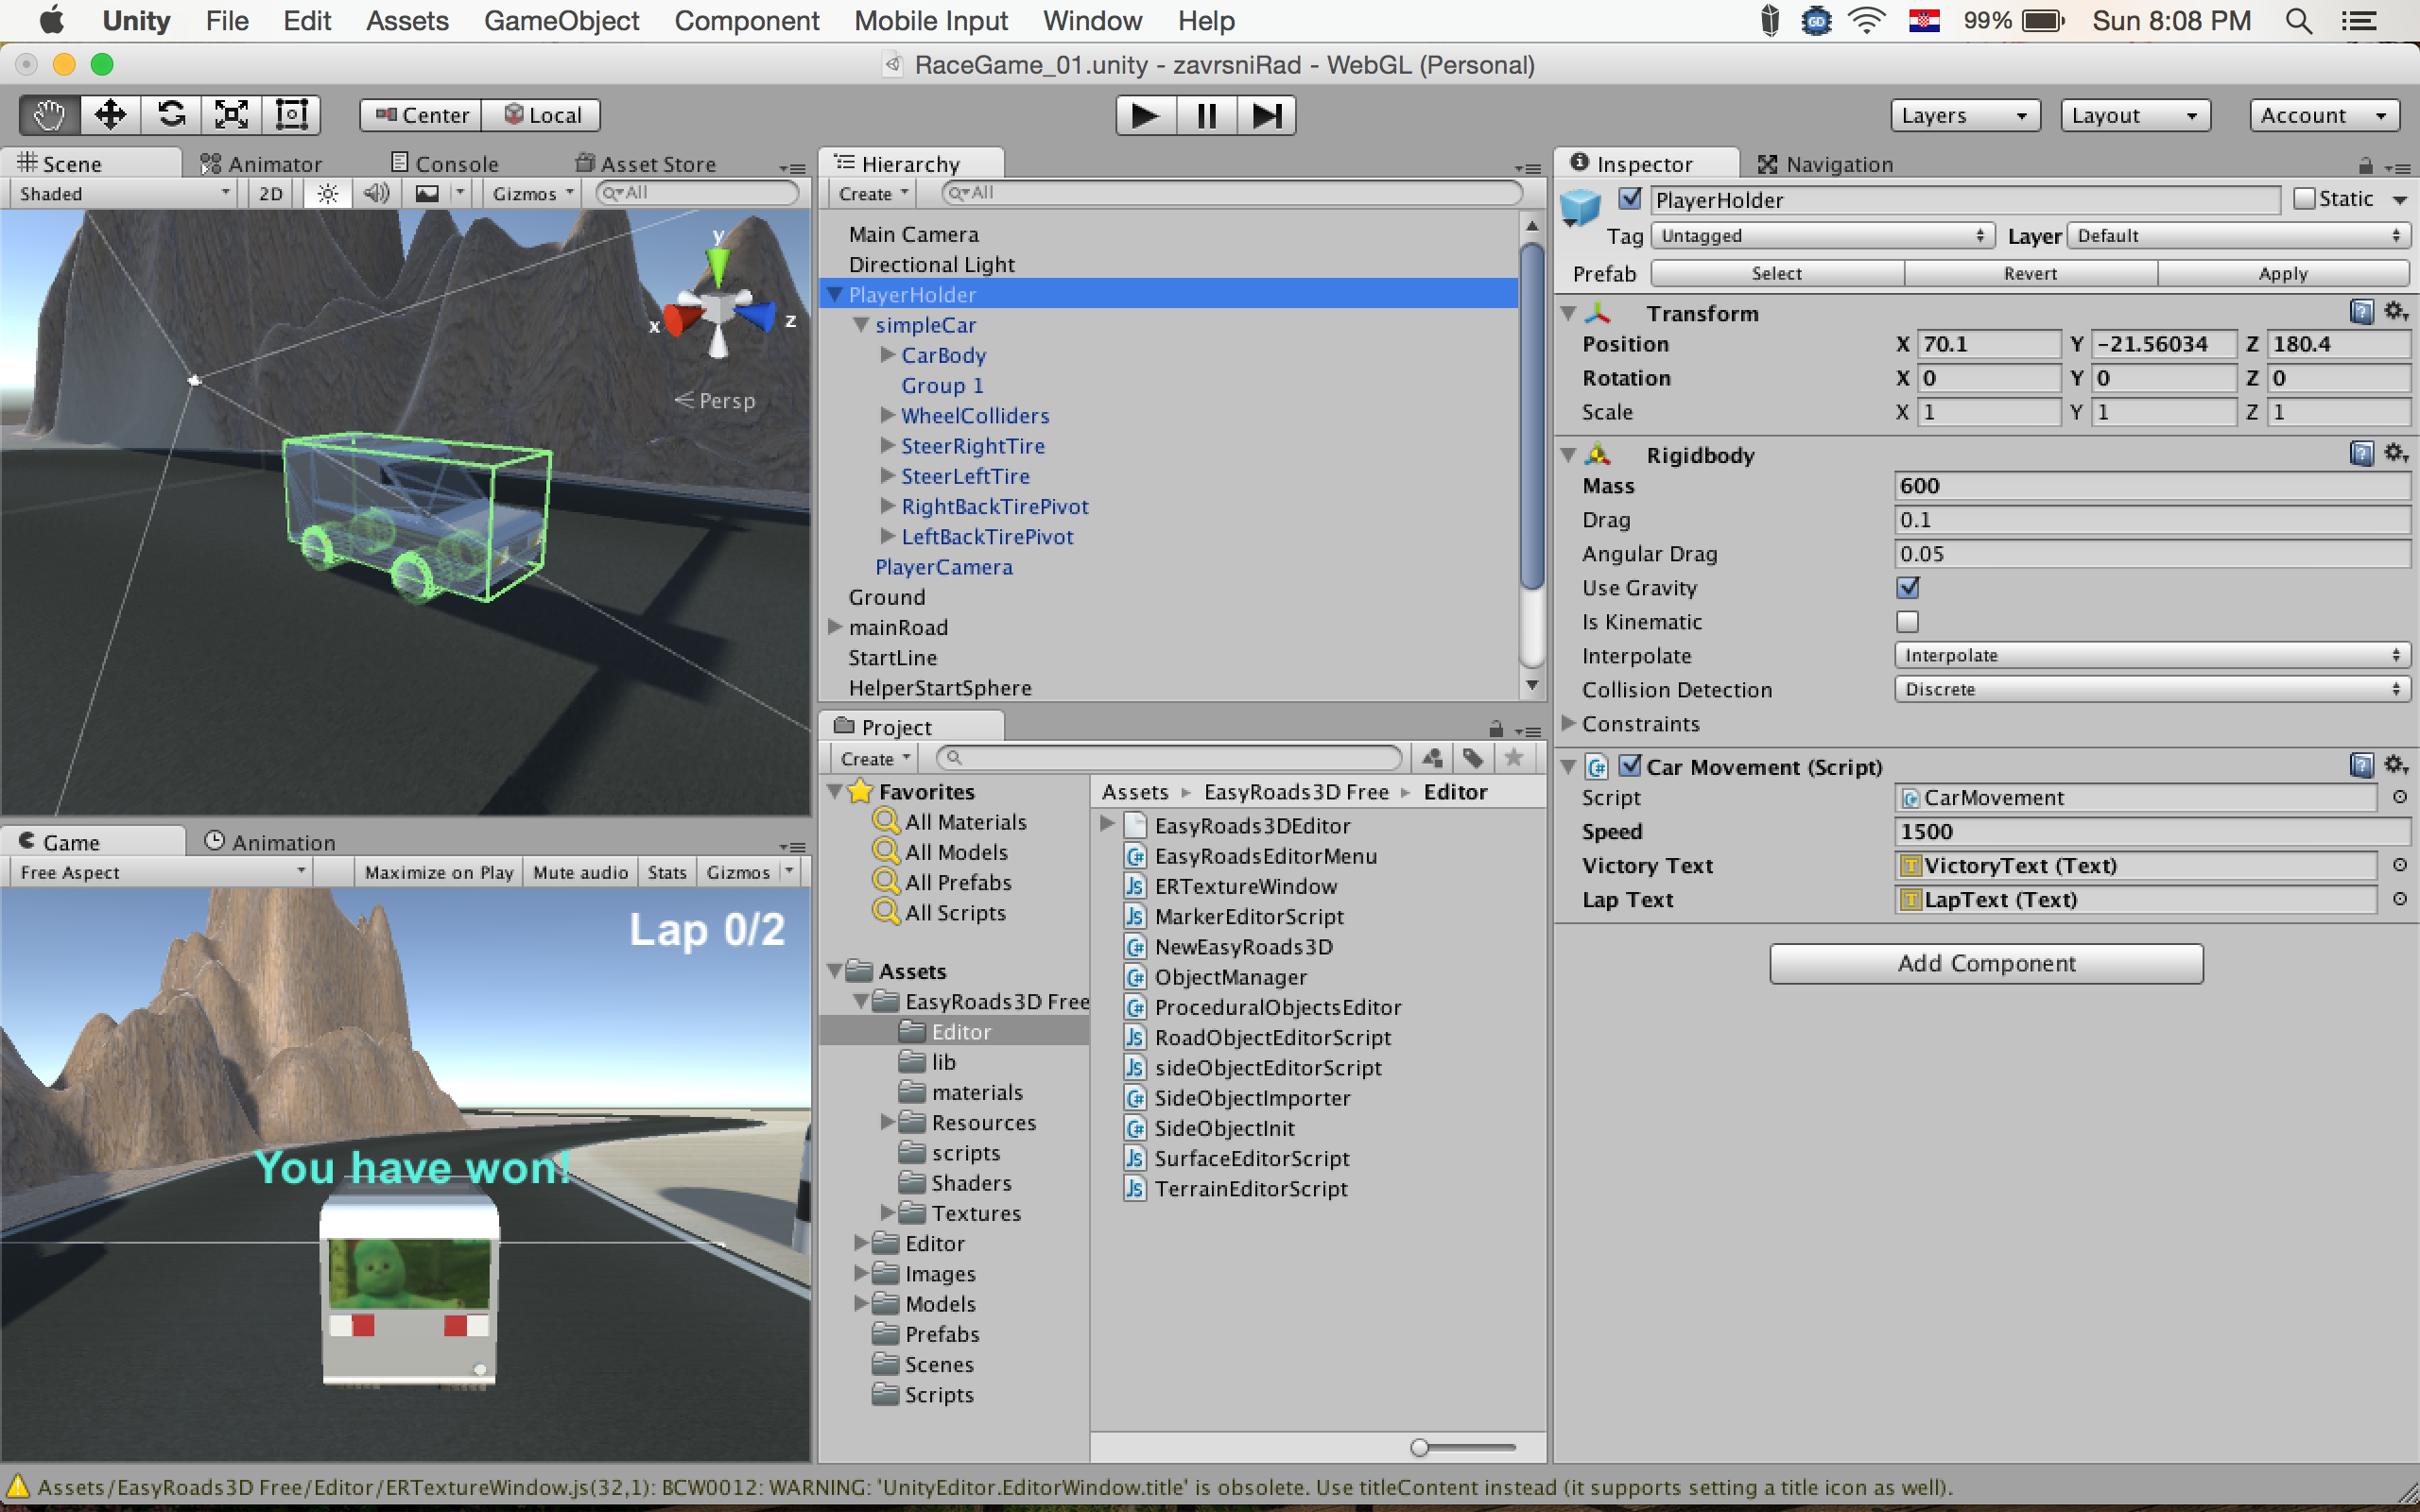
\includegraphics[width=12.5cm, height=10cm]{igrajuci_objekt.png}
	\centering
	\caption{Igrajući objekt}
	\label{fig:igrajuciobjekt}
\end{figure}
\newpage
Na slici broj \ref{fig:igrajuciobjekt} se može vidjeti primjer unity radne okoline i jedan igrajući objekt koji se zove "PlayerHolder". Ovaj igrajući objekt ima tri komponente, transformaciju, kruto tijelo i skriptu koja se zove "CarMovement". O skriptama i kako one funkcioniraju bit će više riječi u sljedećem poglavlju. Dodavanje komponenti se može realizirati klikom na botun "Add Component". Nakon klika na botun se otvara padajući izbornik za odabir željene komponente.

Svaki igrajući objekt pripada jednom sloju (\emph{eng.~Layer}) i ima oznaku (\emph{eng.~Tag}). Kasnije se pomoću skripti može manipulirati ovim elementima provjerom njihovih slojeva i oznaka. U igri se koriste oznake upravo za provjeravanje da li je korisnik prošao cestu pravim putem. Na slici broj \ref{fig:markeriPutanje} se mogu vidjeti markeri koji provjeravaju navedeno.

\subsubsection{Transformacija}
Igrajući objekti moraju imati svoju \textbf{transformaciju}, inače se neće moći prikazati u svijetu. Transformacija definira širinu, poziciju i orijentaciju objekta. Svaka transformacija ima svoj pivot koji određuje centar, odnosno prema njemu se gledaju širina, pozicija i rotacija. Pivot se može gledati globalno ili lokalno. Globalno gledanje je pozicija pivota gledajući koordinate x,y,z svijeta. Lokalno gledanje pivota je relativna pozicija naspram pozicije objekta. Primjer transformacijog elementa (\emph{Gizmo}) se može vidjeti na slici broj \ref{fig:kotaci}.

\subsection{Kotači}

\begin{figure}[h]
	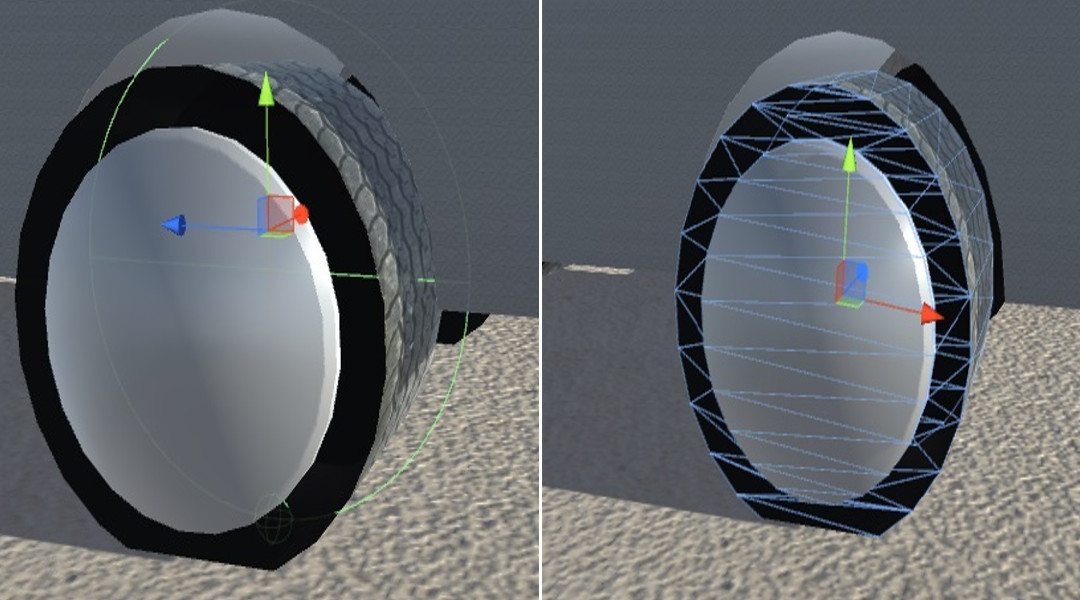
\includegraphics[width=12.5cm, height=7cm]{wheels.jpg}
	\centering
	\caption{Kotači modela}
	\label{fig:kotaci}
\end{figure}

Kako je navedeno u prethodnom poglavlju kotači se sastoje od više komponenti. Te komponente su mreža (\emph{eng.~Mesh}), transformacija, te mrežno renderiranje (\emph{eng.~Mesh Renderer}) koji dopušta korisniku da vidi konačni element. Ono što se koristi za kretanje modela je kolni sudarač. Mreža se može vidjeti na slici \ref{fig:kotaci} desno, a sudarač na slici \ref{fig:kotaci} lijevo. Isto tako veoma bitna stvar je povećati masu modela, inače će početi nekontrolirano rotirati na sceni, kao da je upalo u crnu rupu. Vrijednost mase u konačnici definira kojom silom će gravitacija privlačiti model, odnosno definiramo brzinu. Što je masa veća sporiji je igrajući objekt i obrnuto.

\subsubsection{Rotiranje kotača}
Prilikom vožnje automobila za bolju simulaciju potrebno je okretati i kola. Za isprogramirati ovu naizgled jednostavnu radnju više stvari treba unaprijed biti dobro definirano, inače se stvar komplicira. Ukoliko je igrajući objekt loše definiran i pivoti nisu dobro postavljeni na kotačima, zbog mehanike koju Unity koristi, objekti rotiraju krivo. Da bi se to ispravilo treba koristiti naprednije metode koje povećavaju broj linija k\^oda i stvaraju dodatne probleme. 

Rotacija kotača bi trebala biti oko njegove osi, te se zato mora postaviti pivot u sredinu kotača. Ovo se obavlja tijekom izrade samog modela, te treba paziti na to prije unosa u unity. Ako se pivot nije centrirao prilikom izrade, onda se treba obavljati popravljanje. Koraci za popravljanje:

\begin{enumerate}
	\item Pronaći objekt (kotač) unutar hijerarhije
	\item Napraviti novi prazni objekt na istoj razini kao i kotač
	\item Kotač ubaciti u prazni objekt
\end{enumerate}
Sada za okretanje kotača se koristi novi prazni objekt jer je njegov pivot centriran. Ovakav pristup je jako učestal zbog dizajnera koji ne paze na pivote unutar svojih modela.

\subsubsection{Problemi u zavojima}
Prilikom vožnje vozila dodavanjem samo kolnih sudarača ne bismo dobili potpunu imitaciju pravog vozila. Jedan od problema koji se javlja je preokretanje u zavojima. Ova pojava je sasvim opravdana i nije nikakva greška programa. Što se ustvari događa? Kada vozilo uđe u zavoj i započme skretanje, na njega djeluje centrifugalna sila, podigne se prednji kotač sa tla i kako ne postoji protusila preokrene se. \par
Za ovaj slučaj postoji više rješenja, a onaj koji se koristi u igrici je sljedeći. Pri skretanju se provjeri koji kotač se podiže od tla i na njega se primjeni sila koja djeluje u smjeru gravitacije. Na ovaj način se smanji utjecaj centrifugalne sile, te samim time teže preokrenuti vozilo.